%%
%% Copyright 2007, 2008, 2009 Elsevier Ltd
%%
%% This file is part of the 'Elsarticle Bundle'.
%% ---------------------------------------------
%%
%% It may be distributed under the conditions of the LaTeX Project Public
%% License, either version 1.2 of this license or (at your option) any
%% later version.  The latest version of this license is in
%%    http://www.latex-project.org/lppl.txt
%% and version 1.2 or later is part of all distributions of LaTeX
%% version 1999/12/01 or later.
%%
%% The list of all files belonging to the 'Elsarticle Bundle' is
%% given in the file `manifest.txt'.
%%

%% Template article for Elsevier's document class `elsarticle'
%% with harvard style bibliographic references
%% SP 2008/03/01
%%
%%
%%
%% $Id: elsarticle-template-harv.tex 4 2009-10-24 08:22:58Z rishi $
%%
%%
\documentclass[final,authoryear,11pt,times]{elsarticle}

%% Use the option review to obtain double line spacing
%% \documentclass[authoryear,preprint,review,12pt]{elsarticle}

%% Use the options 1p,twocolumn; 3p; 3p,twocolumn; 5p; or 5p,twocolumn
%% for a journal layout:
%% \documentclass[final,authoryear,1p,times]{elsarticle}
%% \documentclass[final,authoryear,1p,times,twocolumn]{elsarticle}
%% \documentclass[final,authoryear,3p,times]{elsarticle}
%% \documentclass[final,authoryear,3p,times,twocolumn]{elsarticle}

%% \documentclass[final,authoryear,5p,times,twocolumn]{elsarticle}

%% if you use PostScript figures in your article
%% use the graphics package for simple commands
%% \usepackage{graphics}
%% or use the graphicx package for more complicated commands
%% \usepackage{graphicx}
%% or use the epsfig package if you prefer to use the old commands
%% \usepackage{epsfig}

%% The amssymb package provides various useful mathematical symbols
\usepackage{amssymb}

\usepackage[margin=1.25in]{geometry}
\usepackage{bbm}
\usepackage{float}
\usepackage{graphicx}
\usepackage{caption}
\usepackage{subcaption}
\usepackage{cleveref}
\usepackage{csquotes}

\usepackage{setspace}
\onehalfspacing
\usepackage{hyperref}
\hypersetup{
    colorlinks=true,
    linkcolor=blue,
    filecolor=magenta,      
    urlcolor=cyan,
}
\urlstyle{same}

\captionsetup[subfigure]{subrefformat=simple,labelformat=simple}
\renewcommand\thesubfigure{(\alph{subfigure})}

%% The amsthm package provides extended theorem environments
%% \usepackage{amsthm}

%% The lineno packages adds line numbers. Start line numbering with
%% \begin{linenumbers}, end it with \end{linenumbers}. Or switch it on
%% for the whole article with \linenumbers after \end{frontmatter}.
%% \usepackage{lineno}

%% natbib.sty is loaded by default. However, natbib options can be
%% provided with \biboptions{...} command. Following options are
%% valid:

%%   round  -  round parentheses are used (default)
%%   square -  square brackets are used   [option]
%%   curly  -  curly braces are used      {option}
%%   angle  -  angle brackets are used    <option>
%%   semicolon  -  multiple citations separated by semi-colon (default)
%%   colon  - same as semicolon, an earlier confusion
%%   comma  -  separated by comma
%%   authoryear - selects author-year citations (default)
%%   numbers-  selects numerical citations
%%   super  -  numerical citations as superscripts
%%   sort   -  sorts multiple citations according to order in ref. list
%%   sort&compress   -  like sort, but also compresses numerical citations
%%   compress - compresses without sorting
%%   longnamesfirst  -  makes first citation full author list
%%
%% \biboptions{longnamesfirst,comma}

% \biboptions{}
% \setlength{\parskip}{1em}

\journal{cs280r - Final Project Report}

\begin{document}

\begin{frontmatter}

%% Title, authors and addresses

%% use the tnoteref command within \title for footnotes;
%% use the tnotetext command for the associated footnote;
%% use the fnref command within \author or \address for footnotes;
%% use the fntext command for the associated footnote;
%% use the corref command within \author for corresponding author footnotes;
%% use the cortext command for the associated footnote;
%% use the ead command for the email address,
%% and the form \ead[url] for the home page:
%%
%% \title{Title\tnoteref{label1}}
%% \tnotetext[label1]{}
%% \author{Name\corref{cor1}\fnref{label2}}
%% \ead{email address}
%% \ead[url]{home page}
%% \fntext[label2]{}
%% \cortext[cor1]{}
%% \address{Address\fnref{label3}}
%% \fntext[label3]{}

\title{CS280r Final Project Report \\ Voting Rules for Subset Selection}

%% use optional labels to link authors explicitly to addresses:
%% \author[label1,label2]{<author name>}
%% \address[label1]{<address>}
%% \address[label2]{<address>}

\author{Anna Sophie Hilgard and Nicholas Hoernle}


\begin{abstract}
\textit{
Social choice theory, providing tools for making joint decisions in multiagent systems is becoming popular for tasks such as group recommendation systems, information retrieval, and crowdsourcing \citep{moulin2016handbook}. We pose a scenario where a crowd is asked to select a subset of information points regarding a topic and we show that theoretically optimal voting rules are not necessarily applicable to this setting. Rather, we suggest different voting rules place varying amounts of cognitive load on the participants, introducing noise into the votes of the participants and ultimately confounding the results. Our conclusion is that cognitive load should be included as a modeling variable for voting rules that involve subset selection.}

\end{abstract}
\end{frontmatter}

% \linenumbers

%% main text
\section{Introduction}
\label{sec:introduction}
There are interesting settings where humans collaborate with each other and with computers to generate content, including documents (e.g. Wikipedia) \citep{hahn2016knowledge,kittur2013future}, taxonomies \citep{chilton2013cascade} and summaries \citep{khosla2013large}. In multi-agent systems settings where qualitative content is being created or used, it is important to consider the cost of communication. Given a medical setting, \citet{amir2015care} report that study participants could not review necessary information in a timely manner, nullifying the effect of obtaining complete and correct information from others. \citet{hahn2016knowledge} show that crowdsourcing vendors consistently struggle to balance the amount of information needed convey to a worker to fully equip the worker to excel at his/her job without overburdening the process with too much information. An added complication is that in many settings, the ideal contextual information that is shared is subjective. Therefore, multiple parties have competing interests in having their contributions addressed. One possible solution is to allow for a single contributor or an outside controller to make these subjective decisions. However, experiences with content generators with a strong hierarchical or dictatorial leadership \citep{benkler2015peer} have shown that the resulting content is often suboptimal from the viewpoint of the whole and heavily skewed to conform to the opinion(s) of the decision-maker(s). \citet{schwartz2015design} stresses that those situations in which group members have different information and the actions of individuals are interdependent are the most critical to be collectively assessed.

% \subsection{Motivation for Investigation}
% \label{sec:motivation}
Under these conditions, we see a strong case for adopting social budgeting techniques to crowdsource contextual points. Our ultimate goal is to select an ideal set of relevant contextual information while reducing the communication and collaboration overheads that may otherwise be necessary.

\section{Related Work}
\citet{boutilier2015optimal} show that if we assume adopt a utilitarian framework in which we hope to maximize the satisfaction of all group members, properly chosen voting rules can ensure that we minimize the maximum difference between the optimal possible satisfaction to all members and that selected by the voting rule in expectation (the regret). It is clear that for a dictatorial selection, this could be trivially equal to the worst case if the size of the alternative set is larger than two times the size of the set of options to be selected. In particular, we will seek to test the effectiveness of the subset selection algorithm generated by \citet{caragiannis2017subset}, which approaches the problem as a variation on the maximin rule. In particular, the authors show that it is possible to derive an explicit utility function which maximizes regret while maintaining consistency with the votes. We use the following expression for maximum regret for a subset selection $T$:
\begin{equation}\label{eq:max_regret}
\textrm{max}_{S \in A_k} \sum_{i=1}^{n} \frac{\mathbbm{1}[S \succ_{\sigma_i}T]}{\sigma_i(S)}
\end{equation}
Where $S \succ_{\sigma_i}T$ indicates that there is no alternative in T preferred to every alternative in S given the utility function $\sigma_i$. $\sigma_i(S)$ is the ordinal ranking of the best alternative in set $S$ in the ranking determined by the utility function $\sigma_i$. Intuitively, any term in this maximization captures the lost satisfaction to the voters of not having the given set $S_i$ chosen rather than $T$, weighted by how much he or she liked his or her best option in $S_i$. This will lead to a greater penalization for sets $T$ that do not give many participants at least one of their top choices. We seek the set $T$ that minimizes this quantity.
\begin{equation}\label{eq:min_regret}
\textrm{argmin}_{T \in A_k} \textrm{max}_{S \in A_k} \sum_{i=1}^{n} \frac{\mathbbm{1}[S \succ_{\sigma_i}T]}{\sigma_i(S)}
\end{equation}

\citet{caragiannis2017subset} show that this can be solved through an integer linear program (ILP) with $n � m$ variables and $n � m^{2} + {n\choose m}$ constraints, where $n$ is the number of voters and $m$ is the number of alternatives available.

For comparison, we also use plurality/knapsack voting, which has been used in real-world participatory budgeting programs (likely in part because of its computational simplicity and ease of understanding \citeauthor{goel2015knapsack}). Moreover, plurality is shown by \citet{caragiannis2017subset} to have empirical regret approaching that of the subset selection algorithm above for subset sizes greater than three, which will be the case in our experiment and should be generally true for problems of this nature.

We apply these different voting rules to the problem of subset selection and conclude that in practice the success of a voting rule may depend heavily on the difficulty (cognitively or subjectively) one has in comparing options.
%Definition 1 (Comparing Sets). Given a ranking ? ? L and an alternative a ? A, recall that ?(a) denotes the position of a in ?. More generally, for a set S ? A let ?(S) = mina?S ?(a). For sets S,T ? A, we say T ?? S if ?(T) < ?(S), i.e., if there exists an alternative in T that is preferred to every alternative in S in ?.

%The need for such efficient communication was evi- dent in our study: some of the providers we interviewed re- ported that when complete plans or notes are sent to them, they are unable to determine the information most important to consider, and they do not review the information in a timely manner as a result of this information overload. 

%Previous crowdsourc- ing approaches have trouble dealing with cross-topic consis- tency because reading even a single topic can take significant time, let alone reading and editing across all topics.

%These are often ones in which
%individuals must coordinate their actions because their parts of the organization are
%interdependent.

%Correctly specifying an agenda helps to keep meeting topics on track, on time and helps to improve the efficiency and effectiveness of the meeting \citep{schwartz2015design} \citep{lehmann2013sequential}. \citet{schwartz2015design} continues by stating the importance of including items in the agenda that reflect the needs of the individuals in the team. \citet{lehmann2013sequential} assert that unmanaged social interaction leads to poor decision making, ineffective communication and unnecessary conformity. In this light, we have revisited the Care Coordination work presented by \citet{amir2015care} and focus on designing a human-computer collaboration tool that is able to manage the creation of an agenda that is relevant for a diverse team of individuals. \citep{arber2008team} is in agreement with the thesis here that meetings significantly affect the performance of the medical team and on the care that the patient receives. The purpose of this system is to extend \citet{procaccia2016voting} `Voting Rules' framework and text mining techniques to create an initial set of structured agenda items that can then be agreed upon in advance. Furthermore, some of the specific obstacles to efficient teamwork demonstrated in the \citet{amir2015care} study shows that members of the team often find large meetings unproductive and not related to the work that they are doing with the patient. Having a structured agenda in advance will help the team members filter through the potentially time wasting and irrelevant content such that they can address the pertinent issues at hand. Following \citet{schwartz2015design} framework for creating an effective meeting agenda, we propose an agent that is able to source the relevant agenda items, action points and required duration from the team prior to the meeting occurring.
%
%\citep{fatima2004agenda} present a view of negotiations where agents all benefit by reaching an agreement but all have conflicting ideas over how certain tasks should be executed. In a similar way, agents in \citet{amir2015care} medical setting may have differing opinions on the best and most important treatment plans that require discussion, but reaching a feasible agreement in advance... 

\section{Experiment Design}
\label{sec:experiment}
Three voting rules are compared to evaluate the success of the subset selection. To test the voting rules, we pose a setting where participants are requested to select a number of points that may be relevant to a given topic. We compiled a set of 10 supporting points from popular \textit{New York Times} opinion pieces, and used a web-based survey form to allow participants to make subset selections. The topics were presented in a `debate prompt' style and the participants were asked to select the points that would contribute the most value to the presented argument. We also allowed participants to provide feedback on the subset selection styles that they most and least enjoyed (\ref{appendix:qual_feedback}).

\par The interface \footnote{Accessed at: \url{http://nick-and-sophie-harvard-cs280r.s3-website-us-east-1.amazonaws.com/index.html}} was designed to present participants with three questions (on three different articles) and each question displays a different subset selection protocol. The different selection methods include:
\begin{itemize}
\item `ranking' selection by dragging and dropping alternatives into the correct order from most to least useful for the given argument. 
\item `cardinal' selection where each point was given a score out of 10 independently of the others.
\item `plurality' (or knapsack) selection, where check-boxes are selected until 5 selections were made.
\end{itemize}

The study consisted of 37 respondents and 111 subset choices over the three different voting rules. We solve equation \ref{eq:min_regret} using integer linear programming as described by \citet{caragiannis2017subset} to aggregate the ranking and cardinal results into an optimal subset. We induced a ranking over the cardinal results to obtain ranked values to use in the subset selection algorithm, breaking ties at random. For the plurality results, we selected the subset greedily using a majority rule approach. Selected subsets included four points each.

Finally, selected subsets were presented to a different group of 15 participants. These participants were simply asked to select the most relevant subset, given the same topic. This data was also collected through a web-based survey \footnote{Accessed at: \url{http://nick-and-sophie-harvard-cs280r.s3-website-us-east-1.amazonaws.com}}.


\section{Results} 

The results here, while indicative of trends are mostly not statistically significant and thus we do not make \textit{significant} claims about our conclusions. Rather, we use the results to inform interesting questions and to pose further work in this area.

The initial results show a large amount of noise and uncertainty in the selections. Figure \ref{fig:q3raw} shows the score that each answer receives for the third topic \footnote{See \ref{appendix:question_topics} for more details on the specific topics} in the question set under the different voting rules. [\textit{Some useful reference discuss how this uncertainty is expected}]. Simply from the raw data there does not appear to be a large amount of correlation among the voting formats. Table \ref{tbl:voting_aggregation} shows the summary of the selected subsets by the voting aggregation rules explained in \ref{sec:experiment}. Points selected by the various methods showed a generally low degree of overlap. For two of the topics, there was one point present in all three subsets, and for all of the topics, at least two points appeared in multiple subsets. Only one pair of options differed by only a single point.  

\begin{figure}
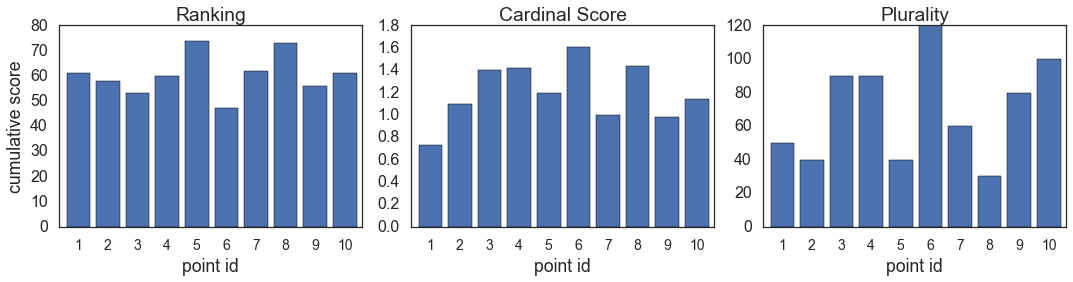
\includegraphics[width=\textwidth, height=3.5cm]{images/question3_raw_results}
\caption{Bar chart of the score each answer point receives under the different voting rules.}
\label{fig:q3raw}
\end{figure}

\begin{table}
\begin{center}
\begin{tabular}{ l | c | c | c }
 & Topic 1 & Topic 2 & Topic 3 \\
 \hline
 \textbf{Ranking}&              $[2, 3, 6, 7]$ & $[2, 3, 7, 10]$ & $[3, 5, 7, 10]$ \\
 \textbf{Cardinal Score}&       $[1, 2, 7, 8]$ & $[4, 7, 8, 10]$ & $[3, 4, 6, 8]$ \\
 \textbf{Plurality Selection}&   $[1, 5, 7, 9]$& $[1, 2, 3, 8]$  & $[3, 4, 6, 10]$ \\
\end{tabular}
\caption{Table showing the selected subset for the different topics for the different voting rules.}
\label{tbl:voting_aggregation}
\end{center}
\end{table}

A different set of voters was asked to vote on qualitatively the best subset. Figure \ref{fig:final_res} shows that the subset from plurality voting produced the most preferred results in all three topics, although for Topic 1 the Cardinal Score was also tied for the most number of votes. The success of simple plurality voting in our experiment over more complicated minimum regret methods leads to a discussion of the appropriateness of minimum regret in our setting. 

\begin{figure}
\centering
\begin{minipage}[t]{.3\textwidth}
		\centering
		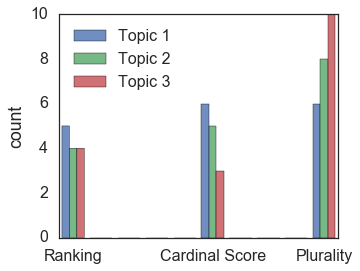
\includegraphics[height=2.5cm]{images/final_results}
		\caption{Bar chart showing the final selected subset for each question for each voting rule.}
		\label{fig:final_res}
  \label{fig:sub1}
\end{minipage}
\hfill
\begin{minipage}[t]{.3\textwidth}
		\centering
		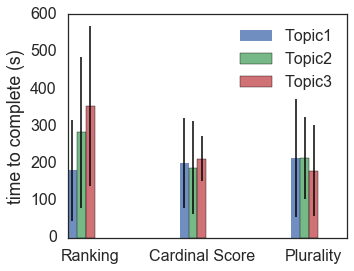
\includegraphics[height=2.5cm]{images/time_to_complete_raw}
		\caption{Time to complete the different voting sections.}
		\label{fig:time_to_complete}
\end{minipage}
\hfill
\begin{minipage}[t]{.3\textwidth}
		\centering
		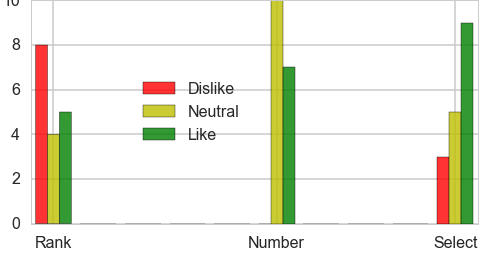
\includegraphics[height=2.5cm]{images/qualitatve_feedback_responses}
		\caption{Chart showing the qualitative sentiment towards the different voting rules.}
		\label{fig:qualitative_feedback}
\end{minipage}
\end{figure}


The time that it took the participants to complete each voting section was recorded. For Topics 2 and 3, the Ranking vote section took on average 1 minute 30 seconds more time to complete than Cardinal and Plurality voting. However, the results from Topic 1 are inconclusive and the standard deviation on the times is large.

Finally, we turn to the qualitative results that were collected in the initial survey. Here we specifically asked participants to provide feedback on the difficulty of the voting rule, and which voting rule they preferred. An example of this feedback is: \textit{``Ranking is the most difficult. I prefer the format that lets me choose on a scale from 1-10 how strong I think the argument is.''} \footnote{All the qualitative feedback is provided in \ref{appendix:qual_feedback}}We parsed the qualitative feedback to understand the sentiment towards the different voting rules. When a specific voting format was mentioned positively or negatively, this was recorded with a $1$ or $-1$ respectively. If the voting rule was not mentioned or was mentioned in a neutral setting the score was recorded as 0. Figure \ref{fig:qualitative_feedback} demonstrates a trend where `Ranking' was disliked more than it was liked, `Plurality' was liked more than it was disliked and `Cardinal Score' shows a neutral-to-positive sentiment. While the preference for a cardinal over an ordinal method runs counter to generally accepted voting design principles, we believe this may have to do with the number of points that must be considered for any given decision as well as some degree of user frustration at inability to assign ties in the ranking. In particular, to properly rank any adjacent pair of points, the user must consider the value of both at once. In assigning a cardinal ranking, the user can focus only on determining the value of a single point.
\section{Discussion}

The results from \citet{caragiannis2017subset} suggest that for a subset of size four, minimum regret should generally provide the lowest upper bound on the regret of participants. That is, it is better in the case where we assume the utility function with highest possible distortion compatible with the selections. However, plurality voting has a very similar upper bound for a subset size of four and may have superior properties in other considerations, as we've seen above. We believe the success of plurality voting in our experiment has to do with two factors.
\subsection{Utility Functions and Separability}
First, the upper bounds assume the worst case separable utility function compatible with the reported rankings. Even in the case where the utility function is in fact separable, this does not imply anything about the average case, and the two worst case bounds are so similar that it is probable that the average case regret for plurality is in fact better. Furthermore, while the points were selected with the quality that they each could stand alone, we see evidence in the data that respondents may be `bundling' points, leading to a different type or problem entirely, and one for which the utility function used in minimum regret is a poor representation of the true utility of voters. Plurality, too, is susceptible to voting paradoxes with nonseparable utility as seen in \citet{moulin2016handbook}, but in our case it seems reasonable that the assumption is approximately true (in that some points may be slightly complementary but the addition of a point should never be detrimental in the presence of other points), and so plurality yields a reasonable approximation of the optimal answer. 

To investigate the presence of this effect in our collected data, we ran a window of length three over every person`s choices, calculating the pairwise distance between all combinations of the three in that window in terms of their ids in our original problem formulation. Because the points were extracted in order from the original opinion pieces (although points are displayed in random order to respondents), numerically close ids correspond to physical and contextual closeness in the original argument. From this, we get an idea of if points that are similar typically get placed with a similar ranking. Figure \ref{fig:pairwise_distance} shows a strong preference for bundling contextually similar points, even though those points are not displayed together in the experiment. In general, \citet{moulin2016handbook} suggests that in fact there are very few domains in which the separability assumption can be expected to hold. In our experiment in particular, it seems likely that human nature pushes respondents to choose a cohesive argument. That is, one in which the arguments made flow well together. The high frequency of a distance of `1' in the figure \ref{fig:pairwise_distance}, corresponding to users selecting points that semantically occurred next to each other in the original article, is significant with a p-value less than [\textit{TODO}].

\begin{figure}
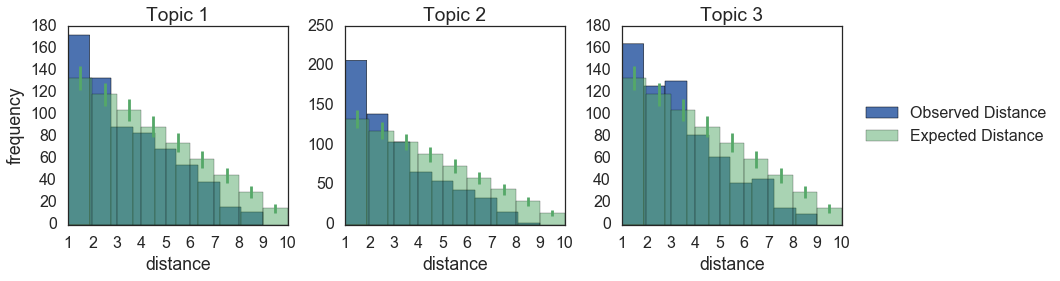
\includegraphics[width=\textwidth, height=3.5cm]{images/pairwise_distance}
\caption{Counts of distances of points in original article when selected in the top or bottom 5 selections.}
\label{fig:pairwise_distance}
\end{figure}


\subsection{Cognitive Load}
Second, our qualitative feedback suggests that knapsack/plurality selection is significantly easier for respondents. This leads us to consider the possible effects of cognitive load on the various voting algorithms. In fact,  \citeauthor{caragiannis2017subset} explicitly mention that the analysis has yet to investigate effects of cognitive load although the authors stress in other works, such as \citet{benade2017preference} that the entire point of a voting mechanisms is to reduce the unacceptable cognitive load of eliciting a full utility function. 

One good reason to do this is that people are likely to make mistakes when presented with a large cognitive load. In particular, in the Sushi dataset from \citet{kamishima2003nantonac}, 70\% of rankings and ratings of the same subsets contain contradictions. That is, the cardinal values in the rating set do not map to the ordinal values in the ranking set. Then it can be assumed that respondents have reported erroneous preferences in one of the two cases, possibly due to excessive cognitive load of the reporting mechanism. If it can be expected that voters will occasionally make errors in reporting their preferences, we should also be interested in the robustness of these selection algorithms to errors. Previous work has shown that the worst case robustness of both minimax and plurality voting is generally better than many other voting methods when considering the worst case for a single winner and that the worst case for a larger subset is bounded by the worst case for a single winner \citep{procaccia2007robustness}. Here, we consider the empirical average case for a variety of subset sizes.

To set up the experiment, we take the Sushi dataset mentioned above and calculate for the rating and ranking problems on the same subsets (these are `sushi3b.5000.10.order' and `sushi3b.5000.10.score') the minimum number of flips of adjacent rankings required to bring the ranking into agreement with a ranking induced over the ratings (flips corresponding to equally rated items are not included in the count, as either ranking of such items is consistent with the rating assuming randomized tie breaking). We tally the distribution of the number of errors throughout all 5000 respondents to the sushi survey. Then, we use the third sushi dataset, `sushi3a.5000.10.order', which contains only 10 types of sushi rather than the 100 in other subsets to bootstrap voting profiles. Because each of the users in the 100 sushi dataset were each only presented with 10 sushi out of the 100, we feel it is fair to assume the same cognitive load would be true for only 10 total sushi types. However, using this dataset allows us to simulate voting over a set of only 10 objects. To create the profiles, we repeatedly draw a set number of voting profiles at random from the rows of the file. We create 100 of these voting profile sets for each trial. Then, we loop through each item in each of the profile sets and induce a number of errors (flips of adjacent rankings) corresponding to a draw from the error distribution. We then perform plurality and minimum regret subset selection on each of the 100 correct voting profile sets and their corresponding profile sets with induced errors and report the number of times the answers matched, in spite of the errors. The results are reported in figures \ref{fig:sub1} and \ref{fig:sub2} for subsets of size 1 to 9 and profile sets of 10 and 20 voters each.

% I believe it is considered better practice to have the graphs at the top of bottom of the pages and then rather link to them.
\begin{figure}
\centering
\begin{minipage}{.5\textwidth}
  \centering
  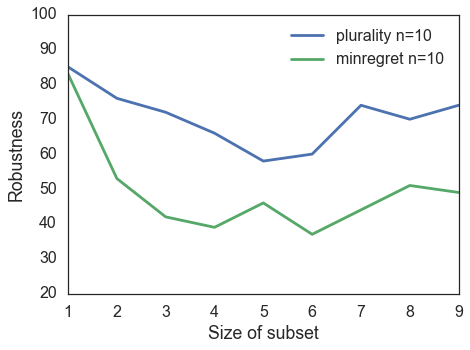
\includegraphics[height=3.5cm]{images/robustness_n10}
  \caption{Robustness with 10 voters and 10 choices}
  \label{fig:sub1}
\end{minipage}%
\begin{minipage}{.5\textwidth}
  \centering
  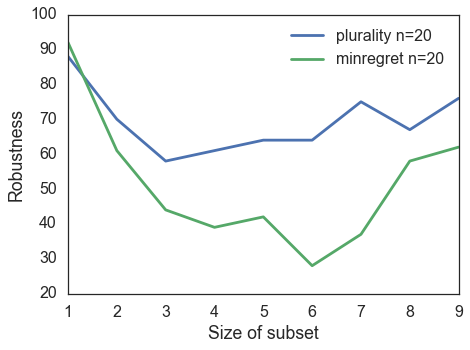
\includegraphics[height=3.5cm]{images/robustness_n20}
\caption{Robustness with 20 voters and 10 choices}\label{fig:sub2}
\end{minipage}
\end{figure}


We find that in general, plurality voting is much more robust to errors in voting than minimum regret. Then, based on our findings, we would expect that the additional cognitive load of ranking induces more errors in voting and that the algorithm is less robust to these errors.


%\subsection{Further Considerations}
%\citet{moulin2016handbook}  mentions four main considerations in evaluation of a voting rule. Communication cost, generality, and quality of the outcome have already been addressed above, in the sections concerning cognitive load, separability, and robustness, respectively. We now also touch briefly on the criterion of computational cost.

\section{Conclusion}
% More generally, even if the assumption of separability were to hold, it is not clear that utilitarian minimum regret should be the objective of choice in content aggregation. Minimum regret may in fact be a better aggregation function for meeting environments, when it is important that all participants have their needs addressed. However, for other content-based applications such as the construction of an argument as above or the composition of a Wikipedia-style article, perhaps it could make more sense to cater to the majority at the expense of minority opinions, depending on the target audience.
%% what happens to quality of outcome when assumptions do not hold
%% generality of approach

With respect to the general field of vote aggregation, our work suggests that assumptions about cognitive load and separability used throughout the literature may be unreasonably favorable. Care should be taken to ensure that any assumptions critical to the evaluation of experiments hold in practice as well as in principle.

Considering content aggregation specifically, we find that the ideal choice of utility and aggregation functions is likely environment-specific. In particular, even if the assumption of separability were to hold, it is not clear that utilitarian minimum regret should be the objective of choice in our content aggregation problem. Minimum regret may in fact be a better aggregation function for environments in which it is important that all participants have their needs addressed. However, for other content-based applications such as the construction of an argument as above or the composition of a Wikipedia-style article, perhaps it could make more sense to cater to the majority at the expense of minority opinions, depending on the target audience.


\section {Future work}
%% explore contexts in which separability is/is not an issue?

% Note that plurality in many cases receives widespread critique as the winner in a voting rule may actually be highly unpopular \citep{moulin2016handbook}, however in the case of subset selection, the distance between different voting options may be small enough to neglect this downfall.

%\subsection{Citations}
%
%Here are two examples of how to cite a paper properly:
%\begin{itemize}
%	\item \citet{bernstein2000complexity} shows that ... 
%	\item Prior work has shown that ... \citep{bernstein2000complexity}.
%\end{itemize}


%%  \citet{key}  ==>>  Jones et al. (1990)
%%  \citep{key}  ==>>  (Jones et al., 1990)


%\section{Related Work}
%Discussion of previous important, similar work in the area with comparison to the particular approach taken and results of the paper. Avoid simply providing a laundry list of other work that is somehow related to the subject of the paper. This section should contain brief, in depth discussions of the work most similar to your project, i.e., to research that takes an approach to the problem or produces results with which your project should be compared. As is always the case with written work, throughout the paper you should have citations to work that you draw on. For example, if you have adapted a system, include a citation to the system when you first mention it; if you are extending a formalization, include a citation to the original on first mention. If you are unclear about whether a simple citation suffices or an extended discussion is needed in the Related Work section, look at the papers read for class this semester for models. If you are still unsure, check with the teaching staff.




%% The Appendices part is started with the command \appendix;
%% appendix sections are then done as normal sections
%% \appendix

%% \section{}
%% \label{}

%% References
%%
%% Following citation commands can be used in the body text:
%%
%%  \citet{key}  ==>>  Jones et al. (1990)
%%  \citep{key}  ==>>  (Jones et al., 1990)
%%
%% Multiple citations as normal:
%% \citep{key1,key2}         ==>> (Jones et al., 1990; Smith, 1989)
%%                            or  (Jones et al., 1990, 1991)
%%                            or  (Jones et al., 1990a,b)
%% \cite{key} is the equivalent of \citet{key} in author-year mode
%%
%% Full author lists may be forced with \citet* or \citep*, e.g.
%%   \citep*{key}            ==>> (Jones, Baker, and Williams, 1990)
%%
%% Optional notes as:
%%   \citep[chap. 2]{key}    ==>> (Jones et al., 1990, chap. 2)
%%   \citep[e.g.,][]{key}    ==>> (e.g., Jones et al., 1990)
%%   \citep[see][pg. 34]{key}==>> (see Jones et al., 1990, pg. 34)
%%  (Note: in standard LaTeX, only one note is allowed, after the ref.
%%   Here, one note is like the standard, two make pre- and post-notes.)
%%
%%   \citealt{key}          ==>> Jones et al. 1990
%%   \citealt*{key}         ==>> Jones, Baker, and Williams 1990
%%   \citealp{key}          ==>> Jones et al., 1990
%%   \citealp*{key}         ==>> Jones, Baker, and Williams, 1990
%%
%% Additional citation possibilities
%%   \citeauthor{key}       ==>> Jones et al.
%%   \citeauthor*{key}      ==>> Jones, Baker, and Williams
%%   \citeyear{key}         ==>> 1990
%%   \citeyearpar{key}      ==>> (1990)
%%   \citetext{priv. comm.} ==>> (priv. comm.)
%%   \citenum{key}          ==>> 11 [non-superscripted]
%% Note: full author lists depends on whether the bib style supports them;
%%       if not, the abbreviated list is printed even when full requested.
%%
%% For names like della Robbia at the start of a sentence, use
%%   \Citet{dRob98}         ==>> Della Robbia (1998)
%%   \Citep{dRob98}         ==>> (Della Robbia, 1998)
%%   \Citeauthor{dRob98}    ==>> Della Robbia


%% References with bibTeX database:

\bibliographystyle{elsarticle-num-names}
\bibliography{bibliography}

\appendix
\section{Qualitative Feedback from Survey}\label{appendix:qual_feedback}

% \appendix
\section{Question Topics}\label{appendix:question_topics}

\end{document}

